
\section{Effizienzoptimierung der Simulationsumgebung} \label{sec:SimEffOpt}
Nach einem Austausch mit dem Forscherteam hinter \emph{RobotSF} wird klar, dass ein
effizientes Training von Fahragenten an erheblichen Effizienzproblemen der
Simulationsumgebung leidet. Die Forscher geben Trainingszeiten von bis zu einem Monat an.
Aufgrund des beschränkten zeitlichen Rahmens dieser Arbeit sind entsprechende Wartezeiten
nicht hinnehmbar, weshalb die Umsetzung durch effizientere Algorithmen und Datenstrukturen
optimiert wird. Zur Messung der Effizienz dient ein Skript, das 10000 Simulationsschritte
ausführt und dabei zufällige Aktionen auswählt. Mithilfe von Scalene
\cite{berger2022triangulating} kann der Beitrag jeder Zeile aus dem Python Quellcode
gemessen werden, um kritische Komponenten zu identifizieren. Anhand der Performance-Profile
ist ersichtlich, dass hauptsächlich der Kraftberechnung von PySocialForce und die
von Caruso et. al umgesetzten Komponenten des LiDAR-Sensors und der Kollisionserkennung
zur Rechenzeit beitragen. Alle restlichen Zeiten werden unter dem Punkt
\glqq{}Sonstige\grqq{} zusammengefasst, wie in Tabelle \ref{tab:SimEffOpt} dargestellt.\\

\begin{table}
\centering
\begin{tabular}{ |p{4cm}||c|c|c|c|c|c| }
 \hline
 Performance-Profil vs. Simulatorversion & Total & PySF & Koll. & LiDAR & Sonst. & Speedup \\
 \hline \hline
 Unoptimized          & 289s & 36\% & 34\% & 19\% & 11\% &  - \\ \hline
 Fast Grid Raycast    & 132s & 76\% & 13\% &  5\% &  6\% & 2.26x \\ \hline
 Fast Grid Map        &  82s & 78\% &  2\% &  9\% & 11\% & 1.61x \\ \hline
 Fast Obstacle Force  &  61s & 74\% &  3\% & 12\% & 11\% & 1.34x \\ \hline
 Continuous Map Algos &  59s & 72\% & 10\% &  6\% & 12\% & 1.03x \\ \hline
 No Custom Forces     &  15s & 30\% &  5\% & 15\% & 50\% & 3.93x \\ \hline
\end{tabular}
\caption{Performance-Profile der jeweiligen Simulatorversionen. Es sind die Gesamtrechenzeit
in Sekunden und die jeweiligen Anteile der Komponenten an der Gesamtzeit in Prozent zu sehen.
Die Spalte \glqq{}Speedup\grqq{} zeigt den jeweiligen Faktor der erzielten Beschleunigung
zur vorherigen Simulatorversion.}
\label{tab:SimEffOpt}
\end{table}

Anhand des ersten Profils entfallen ca. 48\% auf eine Datei namens \glqq{}map.py\grqq{},
die sowohl die Logik zur Kollisionserkennung, als auch die Umsetzung des LiDAR-Sensors
enthält. Daher wird die Repräsentation des Kartenmaterials nun genauer betrachtet. Es stellt
sich heraus, dass die Karte durch eine Rasterstruktur (2D-Bitmaske) umgesetzt wird, wobei
ein Bit pro Zelle angibt, ob sich dort Hindernisse befinden. Zum Aufbau des Rasters werden
die Umrisse aller Entitäten berechnet und anschließend per bitweisem OR zu einer Maske
(engl. Occupancy Grid) zusammengefügt. Umrisse statischer Entitäten werden zu Beginn der
Simulation vorberechet und um die dynamisch berechneten Umrisse aller beweglichen
Entitäten zu jedem Simulationsschritt ergänzt.\\

Vorteile der Datenstruktur bestehen zunächst darin, dass die Komplexität der Algorithmen,
die auf einem fertig berechneten Raster arbeiten, lediglich mit der Rastergröße skaliert,
nicht aber mit der Anzahl der dargestellten Objekte. Die Kollisionsberechnung des
Fahrzeugs kann beispielsweise mittels bitweisem AND der Fahrzeugumrisse mit den
Hindernissen auf der Karte umgesetzt werden. Der Vorteil der Skalierbarkeit ist jedoch
ein Trugschluss, da die Anzahl an simulierten Objekten für einen tatsächlichen Vorteil
größer als die Anzahl der Rasterzellen sein muss. Weitere Nachteile ergeben sich, da das
Sichtfeld des Fahrzeugs mit $O(r^2 d^2)$ bzgl. des Sichtradius $r$ und der Rasterdichte
$d$ skaliert und somit dem \glqq{}Curse of Dimensionality\grqq{} unterliegt, der sich
zudem verstärkt, falls eine feingranularere Rasterisierung der Karte benötigt wird.
Für \emph{RobotSF} wird beispielsweise ein quadratisches Raster mit einer Seitenlänge
von 40 Metern gewählt, dessen Zellen eine Seitenlänge von 0.1 Meter aufwiesen.
Dies entspricht einem Vielfachen von 160000 Rechenzyklen pro Rasteroperation.
Abgesehen von einem erheblichen Verlust an Genauigkeit sind Algorithmen mit Bitmasken
auch sehr ineffizient, da die restlichen Programmteile von \emph{RobotSF} ohnehin mit
Vektorgrafiken arbeiten und daher zu jedem Zeitschritt die Konvertierung aller beweglichen
Objekte in Bitmasken erfordern.
Auch die Umsetzung eines LiDAR-Sensors bzgl. einer Rasterstruktur ist eher umständlich,
da die Strahlen als Pixelgeraden, z.B. mit Bresenham's Line \cite{bresenham65linealgo},
berechnet werden müssen, um dann einen Abgleich der Bitmasken durchführen zu können.
Um die Kompatibilität zur alten Grid-Struktur von Caruso et. al beibehalten zu können, wird
zunächst der LiDAR-Sensor und anschließend die Kollisionserkennung mit Numba optimiert,
indem die Algorithmen dahingehend verbessert werden, möglichst viele Befehle in generierten
C Code auszulagern. Dies führt zu ersten Erfolgen, sodass die Rechenzeiten von vormals 158
Sekunden auf 9 Sekunden gesenkt werden können, was im Bezug auf die Gesamtrechenzeit eine
3.6-fache Beschleunigung erlaubt.\\

Nun stellen die Kraftberechnungen von PySocialForce mit 78\% den Hauptanteil am Profil,
sodass diese im Folgenden näher betrachtet werden. Um den kritischen Pfad von PySocialForce
im Performance-Profil zu analysieren, wird dessen Quelltext von GitHub als Untermodul registriert.
Untersuchungen ergeben, dass 99\% der Rechenzeit für die Abstoßungskraft der Fußgänger von
Hindernissen aufgewendet werden, damit Fußgänger nicht durch diese hindurch laufen können.
Nach genauerer Betrachtung des Codes ergibt sich, wie in Abbildung \ref{fig:ObstacleForceOpt}
dargestellt, dass PySocialForce Hindernisse nicht als
Liniensegmente, sondern als einzelne, zwischen den beiden Endpunkten im Abstand von 0.1 Meter
angeordnete Punkte betrachtet, die zum Simulationsstart vorberechnet werden. Die abstoßende
Kraft wirkt um jeden einzelnen dieser Punkte, wobei die Kraft exponentiell mit wachsender
Entfernung abnimmt. Die Repräsentation von Liniensegmenten durch viele Punkte ist bereits
für kleine Karten sehr ineffizient, da der Algorithmus nicht nur mit der Anzahl der Hindernisse,
sondern zusätzlich mit der Länge der Hindernisse skaliert. Daher wird die Kraftberechnung
durch ein virtuelles Potentialfeld ersetzt, für das die reziproge, quadratische Entfernung
zwischen Fußgängern und Hindernissen aus Abschnitt \ref{sec:SocialForce} herangezogen wird.
Die Formel für die Abstoßungskraft $F = - \frac{\partial}{\partial p} dist(o, p)^{-2}$ entspricht
den partiellen Ableitungen nach der x- und y-Koordinate der Fußgängerposition $p$. Zur Berechnung
der Distanz zwischen Fußgänger und Hindernis kann ein durch $p$ verlaufendes Lot auf das
Liniensegment gefällt werden. Trifft das Lot das Liniensegment nicht, wird stattdessen
die Distanz zum nähergelegenen Endpunkt des Segments herangezogen. Durch diese einfache
Änderung der Berechnungsformel und einige weitere Hardware-Optimierungen mittels Numba
kann die Effizienz des Simulators um Faktor 1.3 gesteigert werden. Des weiteren fällt auf,
dass für einige Kräfte zur Umsetzung von Gruppendynamiken eigene Implementierungen von
Caruso et. al  existieren, die einen sehr großen Anteil am Performance-Profil einnehmen.
Durch das Ersetzen der Kräfte durch ihr standardmäßig in PySocialForce mitgeliefertes
Pendant kann die Simulationszeit nochmals 4-fach beschleunigt werden.\\

\begin{figure}[h]
  \centering
  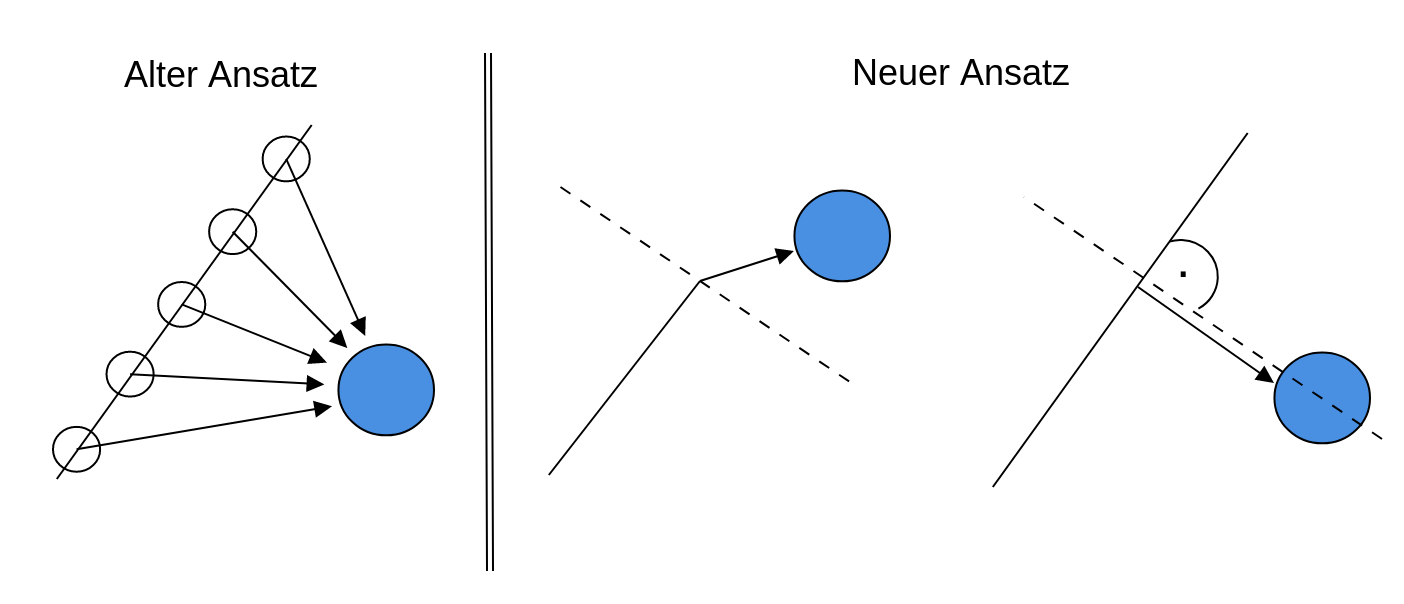
\includegraphics[width = 1.0\textwidth]{imgs/obstacle_force}
  \caption{Umsetzung der \emph{Obstacle Force}. Der alte Ansatz repräsentiert Hindernisse
  als viele Punkte, von denen der Fußgänger jeweils einzeln abgestoßen wird.
  Der neue Ansatz fällt ein Lot auf das Hindernis und stößt den Fußgänger orthogonal ab.
  Befindet sich der Fußgänger neben dem Hindernis, wird die Distanz zum nähergelegenen
  Endpunkt des Hindernisses herangezogen.}
  \label{fig:ObstacleForceOpt}
\end{figure}

Wie bereits angesprochen, ist die Umsetzung der Grid-Struktur sehr unflexibel und verhindert
einfachere Algorithmen mit Vektorgrafiken. Außerdem kann der LiDAR-Sensor aufgrund der
Rundungseffekte durch die Rasterisierung nicht hinreichend getestet werden, um die
Funktionstüchtigkeit der Sensorik sicherzustellen. Aus besagten Gründen wird die Repräsentation
von Hindernissen, Fußgängern, Fahrzeugen und Laserstrahlen auf einfache Vektorgrafiken umgestellt,
wie in Abschnitt \ref{sec:SimEnv} beschrieben. Dies hat zwar keine nennenswerten Auswirkungen auf das
Performance-Profil, aber ermöglicht eine Umstrukturierung und Vereinfachung der Simulationslogik.
Da \emph{RobotSF} nun im Vergleich zur ursprünglichen Simulationsumgebung von Caruso et. al
ungefähr 19-fach beschleunigt ist, können die Trainingsexperimente mit einer vertretretbaren
Wartezeit durchgeführt werden. Es werden noch einige kleinere Verbesserungen eingeführt,
um die Berechnung von Kollisionen und Kräften weit voneinander entfernter Entitäten
zu filtern. Dies soll in diesem Rahmen jedoch nicht weiter thematisiert werden.

\section{Mögliche Verbesserungen bezüglich Effizienz}
Wie der \emph{Mulit-Robot} Ansatz von Fan et. al \cite{fan2020distributed} demonstriert,
können gleichzeitig mehrere Fahrzeuge innerhalb derselben Simulationsumgebung trainieren,
sodass die Umgebung vektorisiert wird. Im Fall von \emph{RobotSF} würde dies zudem eine
Effizienzsteigerung bezüglich der Rechenzeit pro Simulationsschritt ermöglichen, da die
Berechnung der Kinematik und Sensorik pro Fahrzeug nur etwa 12\% Anteil am gesamten
Performance-Profil hat. Je nach Kartenmaterial kann in jeder Startzone je ein Fahrzeug
seine Route starten. Beispielsweise können Fahrzeuge auf dem Universitätscampus an 11
verschiedenen Orten starten, was die während des Trainings verwendeten 64
Simulationsumgebungen auf 6 reduziert. Im konkreten Fall ist in etwa eine 5-fache
Effizienzsteigerung möglich.

$$\eta = \left(\frac{0.88 \cdot 6 + 0.12 \cdot 64}{64}\right)^{-1} \approx 5$$

Durch eine Umstellung auf lokalitätsaffine Algorithmen im Zusammenspiel mit passenden
Datenstrukturen, z.B. Quad-Trees, wie es in der Grafikprogrammierung üblich ist,
sind weitere Effizienzsteigerungen bei der Umsetzung der Simulationsumgebung möglich.
Insbesondere kann die Dimensionierung des simulierten Kartenmaterials aufgrund der
lokalitätsaffinen Algorithmen nochmals deutlich vergrößert werden, sodass mehr
Startplätze und folglich auch weitere Fahrzeuge pro Umgebung denkbar sind.
Eine entsprechende Anpassung der Simulationsumgebung geht über den Umfang dieser Arbeit
deutlich hinaus, kann aber in Anbetracht der möglichen Verbesserungen durchaus
lohnenswert sein, zumal die Ergebnisse von Fan et. al \cite{fan2020distributed} ohnehin eine
Qualitätssteigerung der erlernten Fahrverhaltensweisen in Aussicht stellen.\\

Auch die Umsetzung des Trainingsalgorithmus mit Stable Baselines 3 hat noch
Verbesserungspotential. Während eines Trainingslaufs mit PPO werden ca. 30 Gigabyte
Arbeitsspeicher allokiert. Anhand der 64 parallel betriebenen Simulationen und einem
für das Sammeln der Trainingsdaten verwendeten Zeitintervall von 2048 Simulationsschritten
wären bei optimaler Speichernutzung aber nur ca. 450 Megabyte notwendig. Eine eigene
Implementierung von PPO mit TensorFlow 2 kann erfolgreich die Spiele Pong und CartPole
erlernen, ist jedoch nicht nennenswert effizienter. Um den Speicher adäquat kontrollieren
zu können, wäre eine Portierung hin zu einer hardwarenahen Sprache
sinnvoll. Um den Großteil der Simulationslogik behalten zu können, wird eine graduelle
Umstellung auf Mojo empfohlen. Neben der Unterstützung von eigenem Python Code sind
auch alle verwendeten Abhängigkeiten weiterhin verfügbar. Zusätzlich profitieren
in Mojo geschriebene Programme von einer Hyperparameteroptimierung der Cachegrößen.
Hierzu kompiliert Mojo zur Laufzeit mehrere Versionen des Codes und unterzieht diese
anschließend einigen Benchmarks, sodass eine optimale Performance mit der verwendeten
Maschine ohne tiefe Kenntnisse der Hardwareprogrammierung erzielt werden kann.
